% figures/five-forces.tex
% Standalone TikZ: Porter's Five Forces diagram (ch.11 competitive analysis).
% Compiled to figures/five-forces.pdf via tools/build-figures.sh.
\documentclass[tikz,border=4pt]{standalone}
\usepackage{tikz}
\usetikzlibrary{arrows.meta,positioning,calc}

\definecolor{vcblue}{HTML}{1A5276}
\definecolor{vcteal}{HTML}{0E6655}
\definecolor{vcgray}{HTML}{4D4D4D}

\begin{document}
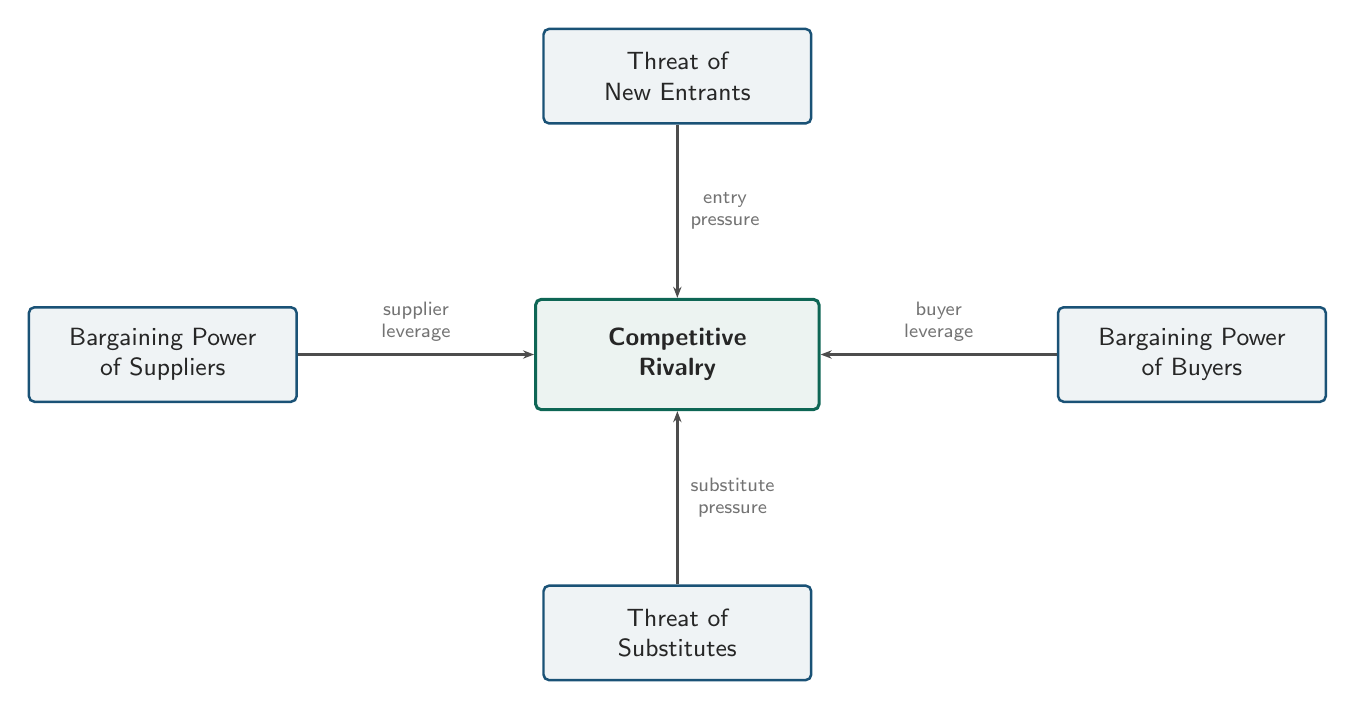
\begin{tikzpicture}[
  node distance=18mm,
  force/.style={draw=vcblue, line width=0.9pt, rounded corners=2pt, fill=vcblue!7,
                font=\sffamily\small, align=center,
                minimum width=34mm, minimum height=12mm, text=black!85},
  rivalry/.style={draw=vcteal, line width=1.1pt, rounded corners=2pt, fill=vcteal!8,
                  font=\sffamily\small\bfseries, align=center,
                  minimum width=36mm, minimum height=14mm, text=black!85},
  arr/.style={-{Stealth[length=4pt]}, vcgray, line width=0.9pt},
  lbl/.style={font=\sffamily\scriptsize, text=black!55, align=center},
]

%% Centre: rivalry
\node[rivalry] (rival) {Competitive\\Rivalry};

%% Four surrounding forces
\node[force, above=22mm of rival] (entry)   {Threat of\\New Entrants};
\node[force, below=22mm of rival] (sub)     {Threat of\\Substitutes};
\node[force, left=30mm of rival]  (supplier){Bargaining Power\\of Suppliers};
\node[force, right=30mm of rival] (buyer)   {Bargaining Power\\of Buyers};

%% Arrows pointing inward toward rivalry
\draw[arr] (entry.south)   -- node[lbl, right=1pt] {entry\\pressure} (rival.north);
\draw[arr] (sub.north)     -- node[lbl, right=1pt] {substitute\\pressure} (rival.south);
\draw[arr] (supplier.east) -- node[lbl, above=1pt] {supplier\\leverage} (rival.west);
\draw[arr] (buyer.west)    -- node[lbl, above=1pt] {buyer\\leverage} (rival.east);

\end{tikzpicture}
\end{document}
